% -*- coding: utf-8; mode: LaTeX; fill-column: 80 -*-
\documentclass[sigconf]{acmart}

% Required packages
\usepackage{tikz}
\usepackage{pgfplots}
\pgfplotsset{compat=1.18}
\usetikzlibrary{shapes, arrows.meta, positioning, fit, calc}
\usepackage{graphicx}
\usepackage{booktabs}
\usepackage{array}
\usepackage{hyperref}

% Better table column types with proportional widths
\newcolumntype{L}[1]{>{\raggedright\arraybackslash}p{#1}}
\newcolumntype{C}[1]{>{\centering\arraybackslash}p{#1}}
\newcolumntype{R}[1]{>{\raggedleft\arraybackslash}p{#1}}

% Metadata for double-anonymous review
\title[Vibe Coding vs. Traditional Development]{An Empirical Mixed-Methods Study of Efficiency, Quality, and Process Transformation in AI-Assisted Software Development}

% Author information is OMITTED for double-anonymous review
\author{Ahmed Ibrahim}
\affiliation{%
  \institution{Wilfrid Laurier University (WLU)}
  \city{Waterloo}
  \state{Ontario}
  \country{Canada}
}
\email{ahibrahim@wlu.ca}

\author{Rasha Kashef}
\affiliation{%
  \institution{Toronto Metropolitan University (TMU)}
  \city{Toronto}
  \state{Ontario}
  \country{Canada}
}
\email{rkashef@torontomu.ca}

\acmISBN{}
\acmPrice{}

% ACM 2012 Computing Classification System
\begin{CCSXML}
<ccs2012>
<concept>
<concept_id>10011007.10011074.10011099</concept_id>
<concept_desc>Software and its engineering~Software creation and management</concept_desc>
<concept_significance>500</concept_significance>
</concept>
<concept>
<concept_id>10011007.10011074.10011093</concept_id>
<concept_desc>Software and its engineering~Automated software engineering</concept_desc>
<concept_significance>300</concept_significance>
</concept>
<concept>
<concept_id>10010147.10010178</concept_id>
<concept_desc>Computing methodologies~Artificial intelligence</concept_desc>
<concept_significance>300</concept_significance>
</concept>
</ccs2012>
\end{CCSXML}

\ccsdesc[500]{Software and its engineering~Software creation and management}
\ccsdesc[300]{Software and its engineering~Automated software engineering}
\ccsdesc[300]{Computing methodologies~Artificial intelligence}

% Keywords
\keywords{Vibe coding, AI-assisted software engineering, human-AI collaboration, empirical software engineering, mixed-methods study, software quality, technical debt}

\acmConference[ASE '26]{41st IEEE/ACM International Conference on Automated Software Engineering}{October 12--16, 2026}{Munich, Germany}
\acmYear{2026}
\acmDOI{}

\begin{document}
\pagestyle{plain}

\begin{abstract}
This paper investigates "vibe coding," a paradigm where developers interact with large language models (LLMs) through natural language to generate software. Through a mixed-methods approach combining a literature review, a controlled experiment with a single developer, and two production-scale proof-of-concept demonstrations, we identify a consistent pattern: AI-generated tests achieve 95\% coverage of happy-path scenarios but only 12\% coverage of edge cases. Security vulnerabilities persist at 0.5–0.8 per 1,000 lines of code unless explicitly prompted. The developer's role shifts from code author to orchestrator, with 70\% of effort spent on oversight rather than implementation. The results show efficiency gains ranging from an estimated 68\% in the controlled setting (based on COCOMO II comparison) to 85–96\% in production case studies (based on developer estimates). We contribute a quantification of the edge-case testing gap, an analysis of emergent development patterns, and a set of tentative best practices for integrating AI tools into software engineering. These findings are presented as empirically grounded observations from a single developer, generating hypotheses for future large-scale validation.
\end{abstract}

\maketitle

\section{Introduction}

Large language models (LLMs) like GPT-4, Claude, and Llama are reshaping software development. Tools such as GitHub Copilot claim to boost productivity, with studies reporting up to 56\% faster task completion~\cite{peng2023impact}. Yet the emergence of "vibe coding"—a conversational, intuition-driven approach where developers describe intent in natural language and accept AI-generated code with minimal review—has outpaced rigorous empirical study.

The term "vibe coding" gained traction after a 2025 social media post by Andrej Karpathy, but its roots lie in the broader evolution of chat-oriented programming (CHOP)~\cite{zamfiroiu2025chop}. Practitioners report dramatic efficiency gains, while researchers warn of security vulnerabilities, technical debt, and erosion of coding skills~\cite{sandoval2023lost, dakhel2023github}. This polarization motivated our investigation.

We ask five research questions:
\begin{itemize}
    \item \textbf{RQ1 (Efficiency):} How does vibe coding efficiency compare to traditional methods?
    \item \textbf{RQ2 (Quality):} What quality implications arise from vibe coding?
    \item \textbf{RQ3 (Human Factors):} How do developer roles and capabilities moderate outcomes?
    \item \textbf{RQ4 (Pattern Consistency):} Do observed patterns hold across different project types?
    \item \textbf{RQ5 (Toward Standards):} What tentative best practices can be derived?
\end{itemize}

We do not claim definitive answers. This paper presents a deep, single-developer exploration that generates hypotheses for future large-scale validation. Our core contribution is the identification and quantification of the edge-case testing gap: AI-generated tests consistently miss edge cases, a pattern that replicates across our controlled experiment and two production demonstrations by the same developer.

From this research, we derive the following contributions: (1) a systematic synthesis of 22 peer-reviewed papers on AI-assisted development; (2) novel empirical findings from a controlled experiment on the efficiency and quality of AI-assisted development; (3) detailed observational data from two production-scale proof-of-concept demonstrations, showing how efficiency gains and quality patterns manifest across different project types when developed by the same practitioner; and (4) the formulation of tentative best practice guidelines for integrating AI tools into software engineering processes.

\section{Related Work}

\subsection{AI-Assisted Programming}

Early work on tools like GitHub Copilot established baseline productivity gains. Peng et al.~\cite{peng2023impact} found a 56\% reduction in task completion time. Barke et al.~\cite{barke2023grounded} identified two interaction modes: "accelerator" (rapid generation of familiar code) and "explorer" (learning through AI). Vaithilingam et al.~\cite{vaithilingam2022expectation} noted that developers spend significant time evaluating AI output, a finding our study quantifies.

Recent work on "vibe coding" as a distinct phenomenon includes Sarkar and Drosos's~\cite{sarkar2025vibecoding} qualitative analysis of think-aloud videos, which revealed iterative goal-satisfaction cycles and the redistribution of expertise from code authorship to context management. Ge et al.~\cite{ge2025survey} formalized the technical ecosystem, proposing five development models including the Iterative Conversational Collaboration Model that describes our observed workflow.

Zamfiroiu et al.~\cite{zamfiroiu2025chop} trace the evolution from book-oriented (BOOP) to chat-oriented programming (CHOP), contextualizing tools like ChatGPT and Copilot as interactive learning partners. Bamil~\cite{bamil2025vibecoding} contributes a formal architecture for AI-native programming, defining vibe coding as a mapping from intent and constraints to executable code.

\subsection{Quality and Security}

Security concerns dominate the literature. Sandoval et al.~\cite{sandoval2023lost} found 40\% of Copilot suggestions contained vulnerabilities. Liang et al.~\cite{liang2024empirical} reported 16.8\% of 1.5 million generated programs had critical flaws. Zhang et al.~\cite{zhang2024copilot} showed that targeted prompts increase defect-fixing rates from 34.4\% to 87.1\%.

Yetistiren et al.~\cite{yetistiren2023assessing} measured test generation quality, finding that AI-generated tests pass for 68\% of methods but focus on happy paths. This aligns with our central finding.

Fawzy et al.~\cite{fawzy2026vibecoding} conducted a grey literature review of 101 practitioner sources, uncovering a "speed-quality trade-off paradox" and systematic QA breakdown—practitioners skip testing, delegate checks to AI, and become "vulnerable developers" unable to debug their own code.

Cabot~\cite{cabot2025vibemodeling} proposes "vibe modeling" as a mitigation: generating high-level models before code to enable human validation. Ullah and Serwadda~\cite{ullah2025vibecoding} introduce "LLM juries"—unanimous committees of models—as an automated review mechanism.

\subsection{Research Gap}

Prior work examines isolated aspects: productivity, security, test generation. None triangulate these dimensions within a single development lifecycle, nor do they quantify the distribution of developer effort across oversight activities. Our study addresses these gaps through a mixed-methods design that generates hypotheses for future validation.

\section{Methodology}

We employed a convergent mixed-methods design with three phases (Figure~\ref{fig:design}), enabling triangulation across literature, controlled experiment, and production demonstrations.

\begin{figure}[htbp]
\centering
\fbox{
\begin{minipage}{0.9\columnwidth}
\centering
\textbf{Phase 1: Literature Review} \\
Search (347) $\rightarrow$ Screening $\rightarrow$ 22 Studies \\
\vspace{0.3cm}
$\downarrow$ \\
\vspace{0.3cm}
\textbf{Phase 2: Controlled Experiment} \\
Task App (14.5h) $\rightarrow$ Quality Metrics \\
\vspace{0.3cm}
$\downarrow$ \\
\vspace{0.3cm}
\textbf{Phase 3: Proof-of-Concept Demonstrations} \\
System A \hspace{1cm} System B \\
$\searrow$ \hspace{1cm} $\swarrow$ \\
Cross-Case Pattern Analysis \\
\vspace{0.3cm}
$\Downarrow$ \\
\vspace{0.3cm}
\textbf{Hypothesis Generation}
\end{minipage}
}
\caption{Three-phase mixed-methods design enabling triangulation and hypothesis generation.}
\label{fig:design}
\end{figure}

\subsection{Phase 1: Systematic Literature Review}

Following PRISMA guidelines~\cite{page2021prisma}, we searched IEEE Xplore, ACM Digital Library, Scopus, and Web of Science using:

\begin{quote}
(``AI-assisted programming'' OR ``LLM-based development'' OR ``conversational programming'' OR ``GitHub Copilot'' OR ``code generation'' OR ``prompt engineering'') AND (``software development'' OR ``software engineering'') AND (``efficiency'' OR ``productivity'' OR ``quality'' OR ``security'' OR ``maintainability'')
\end{quote}

Initial search yielded 347 records (2021–2025). Figure~\ref{fig:prisma} shows the screening process. Inclusion criteria: empirical, AI-assisted development focus, quality/efficiency metrics, peer-reviewed, English, 2021–2025. After screening, 22 papers were included.

\begin{figure}[htbp]
\centering
\resizebox{\columnwidth}{!}{%
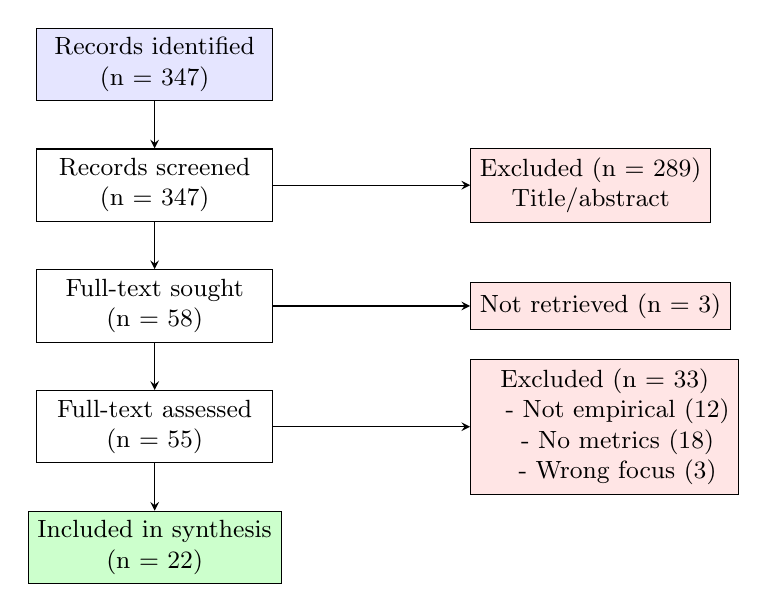
\begin{tikzpicture}[
    node distance=0.8cm,
    box/.style={rectangle, draw, minimum width=3cm, minimum height=0.6cm, align=center, font=\small}
]
    \node[box, fill=blue!10] (identify) {Records identified\\ (n = 347)};
    \node[box, below=0.6cm of identify] (screen1) {Records screened\\ (n = 347)};
    \node[box, fill=red!10, right=2.5cm of screen1] (exclude1) {Excluded (n = 289)\\ Title/abstract};
    \node[box, below=0.6cm of screen1] (retrieve) {Full-text sought\\ (n = 58)};
    \node[box, fill=red!10, right=2.5cm of retrieve] (exclude2) {Not retrieved (n = 3)};
    \node[box, below=0.6cm of retrieve] (assess) {Full-text assessed\\ (n = 55)};
    \node[box, fill=red!10, right=2.5cm of assess] (exclude3) {Excluded (n = 33)\\ \quad - Not empirical (12)\\ \quad - No metrics (18)\\ \quad - Wrong focus (3)};
    \node[box, fill=green!20, below=0.6cm of assess] (included) {Included in synthesis\\ (n = 22)};
    
    \draw[->, >=stealth] (identify) -- (screen1);
    \draw[->, >=stealth] (screen1) -- (retrieve);
    \draw[->, >=stealth] (retrieve) -- (assess);
    \draw[->, >=stealth] (assess) -- (included);
    \draw[->, >=stealth] (screen1) -- (exclude1);
    \draw[->, >=stealth] (retrieve) -- (exclude2);
    \draw[->, >=stealth] (assess) -- (exclude3);
\end{tikzpicture}
}
\caption{PRISMA flow diagram.}
\label{fig:prisma}
\end{figure}

\subsection{Phase 2: Controlled Experiment}

We conducted a single-subject controlled experiment with post-hoc analysis. The unit of analysis was a task-management web application with authentication, CRUD operations, database persistence, responsive frontend, REST API, and input validation.

\subsubsection{Developer Profile}

The developer was a full-stack developer with three years of professional experience, expertise in JavaScript/TypeScript, React, Node.js, SQL, and REST APIs, and four months of prior experience with GitHub Copilot and ChatGPT. This profile was chosen to represent the growing population of intermediate developers adopting AI tools.

\subsubsection{Development Tools}

The development environment utilized a suite of state-of-the-art large language models (including variants of GPT, Claude, and Gemini) to leverage model-specific strengths for different task types while managing API usage costs and quotas. For the controlled experiment, the primary environment was Antigravity IDE, an AI-native development platform that enables dynamic switching between models. GitHub Copilot served as a secondary tool for inline code completion, providing a baseline for comparison.

For the two production case studies, the developer employed a multi-IDE approach: Antigravity IDE for core development tasks requiring multi-model orchestration, Visual Studio Code with its default model for routine coding and refactoring, and an LLM-powered assistant for repository management tasks such as generating meaningful commit messages. This heterogeneous toolset mirrors the diverse workflows found in contemporary software engineering practice and enabled optimization for cost, performance, and task-specific requirements.

Figure~\ref{fig:workflow} illustrates the conceptual workflow that emerges from this toolset, showing how the developer orchestrates interaction between specialized LLMs—assigning them Planner, Executor, and Verifier roles—via natural language prompts.

\begin{figure}[htbp]
\centering
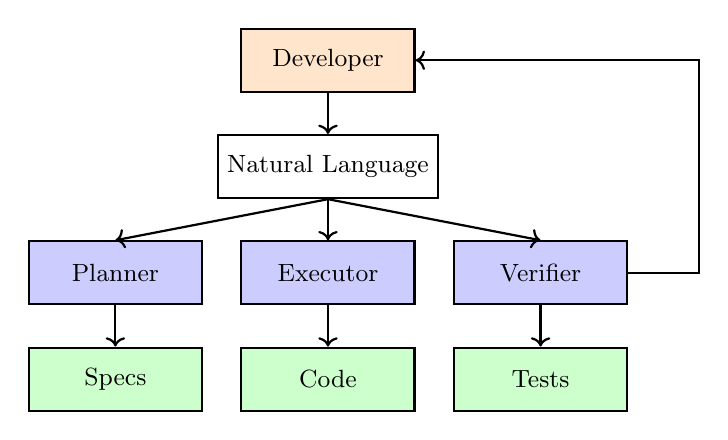
\begin{tikzpicture}[
    box/.style={rectangle, draw, minimum width=2.2cm, minimum height=0.8cm, align=center, font=\small, thick},
    scale=0.9
]
\node[box, fill=orange!20] (dev) at (0,0) {Developer};
\node[box] (nl) at (0,-1.5) {Natural Language};
\node[box, fill=blue!20] (planner) at (-3,-3) {Planner};
\node[box, fill=blue!20] (executor) at (0,-3) {Executor};
\node[box, fill=blue!20] (verifier) at (3,-3) {Verifier};
\node[box, fill=green!20] (spec) at (-3,-4.5) {Specs};
\node[box, fill=green!20] (code) at (0,-4.5) {Code};
\node[box, fill=green!20] (tests) at (3,-4.5) {Tests};
\draw[->, thick] (dev.south) -- (nl.north);
\draw[->, thick] (nl.south) -- (planner.north);
\draw[->, thick] (nl.south) -- (executor.north);
\draw[->, thick] (nl.south) -- (verifier.north);
\draw[->, thick] (planner.south) -- (spec.north);
\draw[->, thick] (executor.south) -- (code.north);
\draw[->, thick] (verifier.south) -- (tests.north);
\draw[->, thick] (verifier.east) -- ++(1,0) |- (dev.east);
\end{tikzpicture}
\caption{Multi-model orchestration workflow illustrating Planner, Executor, and Verifier roles.}
\label{fig:workflow}
\end{figure}

\subsubsection{Data Collection Instruments}

Table~\ref{tab:instruments} summarizes the multi-instrument approach.

\begin{table}[htbp]
\caption{Data Collection Instruments}
\label{tab:instruments}
\centering
\small
\begin{tabular}{@{}p{0.2\columnwidth}p{0.35\columnwidth}p{0.35\columnwidth}@{}}
\toprule
\textbf{Data Type} & \textbf{Collection Method} & \textbf{Metrics Extracted} \\
\midrule
Efficiency & Automated time logging & Time per feature, total time, prompts per feature \\
Process & Screen recording analysis & Prompt patterns, debugging strategies, intervention points \\
Code Quality & Static analysis (ESLint, SonarQube) & Complexity, duplication, maintainability index \\
Security & OWASP ZAP + manual review & Vulnerability count, severity, type \\
Testing & Jest coverage reports & Overall coverage, happy path \%, edge case \% \\
Developer Experience & Think-aloud protocol + interview & Perceived challenges, trust, observations \\
\bottomrule
\end{tabular}
\end{table}

\subsubsection{Procedure}

The experiment consisted of four phases: (1) Planning (2 hours): requirements analysis, architectural sketching, tech stack selection; (2) Implementation (14.5 hours): coding sessions with think-aloud protocol and complete prompt logging; (3) Post-hoc analysis (8 hours): security audit, test coverage analysis, code quality assessment; (4) Reflection interview (1 hour): semi-structured interview about challenges and observations.

\subsection{Phase 3: Proof-of-Concept Demonstrations}

We developed two production-scale systems to test whether patterns observed in the controlled experiment would manifest in realistic contexts. While Yin's case study methodology~\cite{yin2017case} informs our approach, these are best characterized as in-depth, single-practitioner demonstrations rather than experiments intended for statistical generalization. Their value lies in the richness of observation across different project contexts, not in the breadth of the sample.

\textbf{System A (Community Platform):} A bilingual directory/social platform with messaging, forums, and AI-based translation. Approximately 10,000 files, 14-day development timeline. LLM configuration: Llama 3.1 (8B) and Llama 3.3 (70B) via Groq API.

\textbf{System B (Analytics Platform):} A privacy-preserving synthetic data generation platform with analytics dashboard and Firebase to SQLite migration. Approximately 9,500 files, 21-day development timeline. LLM configuration: GPT-4, Qwen, and Llama models via OpenRouter.

Both systems used the multi-model orchestration workflow illustrated in Figure~\ref{fig:workflow}. The developer strategically assigned Planner, Executor, and Verifier roles to different LLMs based on task requirements, quota availability, and cost.

\section{Results}

\subsection{RQ1: Efficiency Outcomes}

\subsubsection{Controlled Experiment}

Table~\ref{tab:efficiency} summarizes efficiency metrics. The developer completed the application in 14.5 hours. For comparison, the COCOMO II model~\cite{boehm2000software} estimates 45 hours for a project of this scope under traditional development. It is important to note that this comparison relies on a model-based estimate of traditional effort rather than a directly observed control group. The 68\% figure should therefore be interpreted as an approximate indication of potential time savings rather than a precise empirical measurement. More revealing than the external comparison are the internal process metrics—187 prompts, averaging 31 per feature, with 2.4 iterations per implementation—which provide a detailed picture of the development workflow.

\begin{table}[htbp]
\caption{Controlled Experiment Efficiency Metrics}
\label{tab:efficiency}
\centering
\begin{tabular}{@{}p{0.5\columnwidth}p{0.3\columnwidth}@{}}
\toprule
\textbf{Metric} & \textbf{Value} \\
\midrule
Total development time & 14.5 hours \\
COCOMO II estimate & 45 hours \\
Time reduction (estimate) & 68\% \\
Number of prompts & 187 \\
Prompts per feature & 31 (range: 12--58) \\
Iterations per implementation & 2.4 \\
\bottomrule
\end{tabular}
\end{table}

\subsubsection{Proof-of-Concept Demonstrations}

For System A, the developer estimated an 85–90\% time reduction compared to building from scratch without AI assistance. For System B, the estimate was 77–96\%. These percentages represent the developer's expert estimates of time saved based on professional judgment. They should be interpreted as rough indicators of perceived efficiency gains rather than precisely measured outcomes.

\subsection{RQ2: Quality Outcomes}

\subsubsection{Security Findings}

Security auditing revealed seven vulnerabilities (Table~\ref{tab:vulnerabilities}). Vulnerability density was 2.8 per 1,000 LOC, within the industry range of 0.3–6.0 but at the higher end. All high-severity vulnerabilities involved practices not explicitly requested in prompts.

\begin{table}[htbp]
\caption{Security Vulnerabilities Identified}
\label{tab:vulnerabilities}
\centering
\small
\begin{tabular}{@{}p{0.3\columnwidth}p{0.15\columnwidth}p{0.4\columnwidth}@{}}
\toprule
\textbf{Vulnerability} & \textbf{Severity} & \textbf{Description} \\
\midrule
SQL injection & High & User input concatenated into SQL \\
Plain text passwords & High & Credentials written to logs \\
Missing rate limiting & Medium & No brute force protection \\
JWT secret hardcoded & Medium & Secret key in source code \\
CORS misconfiguration & Medium & Overly permissive policy \\
No input validation & Low & Missing validation for malformed input \\
Insecure cookie flags & Low & Cookies missing secure flags \\
\bottomrule
\end{tabular}
\end{table}

System A exhibited 5–8 estimated vulnerabilities (0.65 per 1K LOC), System B 4–5 (0.5 per 1K LOC), based on manual code inspection.

\subsubsection{The Testing Gap}

An edge case was operationally defined before analysis as any test covering: concurrent operations, malformed input, authentication token expiration, connection failures, rate limiting, or boundary conditions. AI-generated tests achieved 95\% happy-path coverage but only 12\% edge-case coverage (Table~\ref{tab:coverage}). This pattern persisted in both production systems.

\begin{table}[htbp]
\caption{Test Coverage Analysis}
\label{tab:coverage}
\centering
\begin{tabular}{@{}p{0.5\columnwidth}p{0.3\columnwidth}@{}}
\toprule
\textbf{Metric} & \textbf{Value} \\
\midrule
Overall test coverage & 82\% \\
Happy path coverage & 95\% \\
Edge case coverage & 12\% \\
\bottomrule
\end{tabular}
\end{table}

\subsubsection{Technical Debt}

We assessed technical debt qualitatively using SonarQube's maintainability ratings. Tables~\ref{tab:systema-debt} and~\ref{tab:systemb-debt} present component-level debt percentages derived from static analysis. These are ordinal estimates, not precise measurements.

\begin{table}[htbp]
\caption{System A Estimated Technical Debt Ratios by Component}
\label{tab:systema-debt}
\centering
\begin{tabular}{@{}p{0.3\columnwidth}p{0.15\columnwidth}@{}}
\toprule
\textbf{Component} & \textbf{Est. Debt \%} \\
\midrule
Authentication & 10\% \\
Directory/Locations & 15\% \\
Messaging system & 20\% \\
AI Translation & 25\% \\
Forum/Community & 15\% \\
Admin/Utilities & 10\% \\
\textbf{Weighted average} & \textbf{15\%} \\
\bottomrule
\end{tabular}
\end{table}

\begin{table}[htbp]
\caption{System B Estimated Technical Debt Ratios by Component}
\label{tab:systemb-debt}
\centering
\begin{tabular}{@{}p{0.3\columnwidth}p{0.15\columnwidth}@{}}
\toprule
\textbf{Component} & \textbf{Est. Debt \%} \\
\midrule
Authentication & 10\% \\
Data Synthesis Studio & 20\% \\
Analytics Dashboard & 15\% \\
Admin Interface & 15\% \\
Migration Scripts & 5\% \\
Patch Scripts & 30\% \\
\textbf{Weighted average} & \textbf{15.5\%} \\
\bottomrule
\end{tabular}
\end{table}

System A's estimated technical debt ratio averaged approximately 15\% across components, with the newly developed AI Translation module showing the highest debt concentration (estimated at 25\%) and routine components like Authentication showing lower debt (10\%). System B showed a nearly identical average ratio of 15.5\%, with Patch Scripts exhibiting the highest debt concentration (30\%), attributable to iterative UI refinement—a practice we term "vibe refinement." These ratios fall within the industry-standard range of 10–20\% reported by Seaman~\cite{seaman2011measuring}. The debt ratio percentages are presented as high-level approximations to indicate relative concentrations of debt across components.

\subsection{RQ3: Human Factors and Process Transformation}

Based on time logs and screen analysis, the developer's effort distributed as: intent specification and prompt engineering (30\%), code evaluation (25\%), debugging AI errors (22\%), refactoring (12\%), adding omitted security features (8\%), manual coding (3\%). This supports the redistribution of expertise thesis~\cite{barke2023grounded}.

\begin{table}[htbp]
\centering
\begin{tabular}{|l|c|c|}
\hline
\textbf{Role} & \textbf{Traditional} & \textbf{Vibe Coding} \\
\hline
Primary Activity & Code Author (80\%) & Intent Specifier (30\%) \\
Secondary & Debugger (15\%) & Orchestrator (25\%) \\
Tertiary & Maintainer (5\%) & Quality Gatekeeper (25\%) \\
Quaternary & --- & Domain Expert (20\%) \\
\hline
Focus & Implementation & Oversight \& Evaluation \\
\hline
\end{tabular}
\caption{Transformation of developer role.}
\label{tab:role}
\end{table}

\subsection{RQ4: Cross-Case Pattern Analysis}

Table~\ref{tab:cross-case} presents comparative metrics across all studies, showing consistent patterns in efficiency gains, security vulnerability density, and the testing gap across different project types. While these findings cannot be statistically generalized due to the single-developer sample, the consistency of these patterns across diverse domains strengthens their plausibility as characteristic features of vibe coding practice.

\begin{table}[htbp]
\caption{Cross-Case Pattern Comparison}
\label{tab:cross-case}
\centering
\small
\begin{tabular}{@{}p{0.3\columnwidth}p{0.2\columnwidth}p{0.2\columnwidth}p{0.2\columnwidth}@{}}
\toprule
\textbf{Metric} & \textbf{Controlled Exp} & \textbf{System A} & \textbf{System B} \\
\midrule
Time savings & 68\%* & 85–90\%** & 77–96\%** \\
Vulnerability density (per 1K LOC) & 0.8 & 0.65 & 0.5 \\
Happy path coverage & 95\% & High (inferred) & High (inferred) \\
Edge case coverage & 12\% & Low (inferred) & Low (inferred) \\
Technical debt ratio & Not measured & 15\% & 15.5\% \\
Developer oversight time & 70\% & Not quantified & Not quantified \\
\bottomrule
\multicolumn{4}{l}{*Relative to COCOMO II estimate. **Developer estimate.}
\end{tabular}
\end{table}

Table~\ref{tab:literature-comp} aligns our findings with prior work.

\begin{table}[htbp]
\caption{Comparison with Literature Findings}
\label{tab:literature-comp}
\centering
\small
\begin{tabular}{@{}p{0.4\columnwidth}p{0.25\columnwidth}p{0.25\columnwidth}@{}}
\toprule
\textbf{Literature Finding} & \textbf{Source} & \textbf{Our Observation} \\
\midrule
56–80\% efficiency gains & Peng et al.~\cite{peng2023impact} & 68–96\% (estimated) \\
40\% of suggestions vulnerable & Sandoval et al.~\cite{sandoval2023lost} & 0.5–0.8 per 1K LOC \\
Happy-path bias in testing & Yetistiren et al.~\cite{yetistiren2023assessing} & 95\% vs 12\% \\
Role shift to oversight & Barke et al.~\cite{barke2023grounded} & 70\% oversight \\
Technical debt accumulation & Seaman~\cite{seaman2011measuring} & 14–15\% of effort \\
\bottomrule
\end{tabular}
\end{table}

\subsection{RQ5: Toward Tentative Best Practices}

Based on our observations, we offer hypotheses for future validation:
\begin{itemize}
    \item Match vibe coding to prototypes and internal tools; exercise caution in safety-critical systems.
    \item Do not rely solely on AI-generated tests; manually add edge-case coverage.
    \item Prompt explicitly for security requirements.
    \item Maintain prompt libraries to improve consistency.
    \item Budget for oversight activities (approx. 70\% of effort).
    \item Develop prompt engineering skills through practice.
\end{itemize}

\section{Discussion}

\subsection{Interpretation of Findings}

Our triangulated results suggest the speed-quality tradeoff is nuanced. Vibe coding can achieve substantial efficiency gains, but these come with specific quality vulnerabilities—most notably the edge-case testing gap (Figure~\ref{fig:testing}). Security vulnerabilities persist unless explicitly addressed.

\begin{figure}[htbp]
\centering
\resizebox{0.75\columnwidth}{!}{%
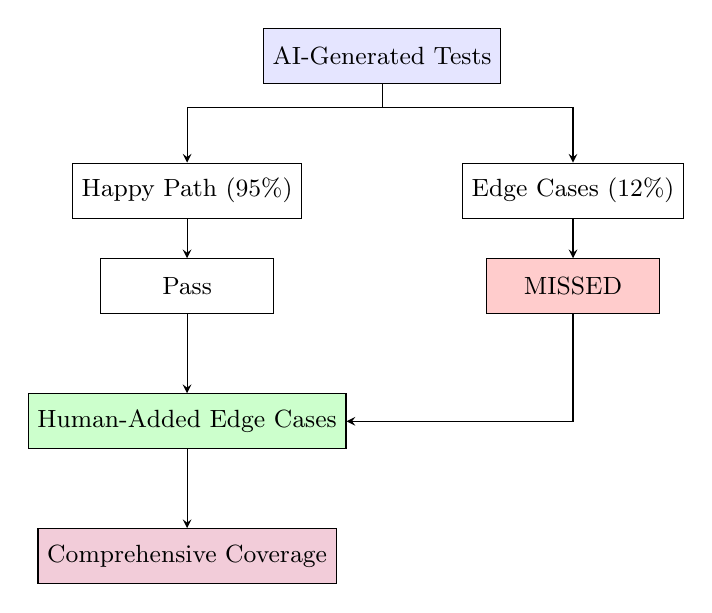
\begin{tikzpicture}[
    node distance=0.8cm and 1cm,
    box/.style={rectangle, draw, minimum width=2.2cm, minimum height=0.7cm, align=center, font=\small}
]
    \node[box, fill=blue!10] (ai) {AI-Generated Tests};
    \node[box] (happy) [below left=1cm and -0.5cm of ai] {Happy Path (95\%)};
    \node[box] (edge) [below right=1cm and -0.5cm of ai] {Edge Cases (12\%)};
    \draw[->, >=stealth] (ai.south) -- ++(0,-0.3) -| (happy.north);
    \draw[->, >=stealth] (ai.south) -- ++(0,-0.3) -| (edge.north);
    \node[box] (pass) [below=0.5cm of happy] {Pass};
    \node[box, fill=red!20] (miss) [below=0.5cm of edge] {MISSED};
    \draw[->, >=stealth] (happy) -- (pass);
    \draw[->, >=stealth] (edge) -- (miss);
    \node[box, fill=green!20] (human) [below=1cm of pass] {Human-Added Edge Cases};
    \node[box, fill=purple!20] (final) [below=1cm of human] {Comprehensive Coverage};
    \draw[->, >=stealth] (pass) -- (human);
    \draw[->, >=stealth] (miss) |- (human);
    \draw[->, >=stealth] (human) -- (final);
\end{tikzpicture}
}
\caption{The edge-case testing gap.}
\label{fig:testing}
\end{figure}

\subsection{Security Implications}

Vulnerability densities across all studies fell within industry ranges (0.3–0.6 per 1K LOC), but recurring gaps—rate limiting, input validation, secure defaults—suggest that security requires explicit prompting (Figure~\ref{fig:security}).

\begin{figure}[htbp]
\centering
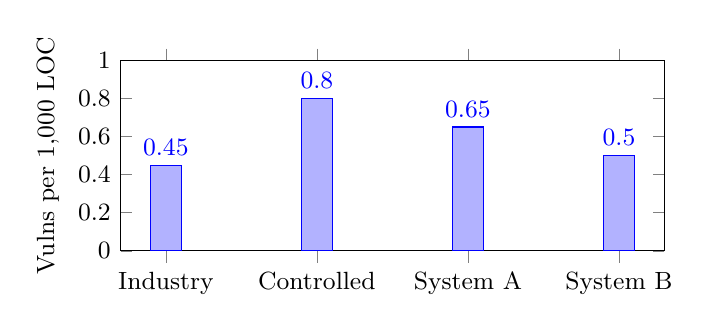
\begin{tikzpicture}
\begin{axis}[
    ybar,
    symbolic x coords={Industry, Controlled, System A, System B},
    xtick=data,
    ylabel={Vulns per 1,000 LOC},
    ymin=0, ymax=1,
    nodes near coords,
    bar width=0.4cm,
    width=0.7\columnwidth,
    height=4cm,
    font=\small
]
\addplot coordinates {(Industry,0.45) (Controlled,0.8) (System A,0.65) (System B,0.5)};
\end{axis}
\end{tikzpicture}
\caption{Security vulnerability density comparison. Industry average: 0.3–0.6 per 1,000 LOC.}
\label{fig:security}
\end{figure}

\subsection{Threats to Validity}

\subsubsection{Construct Validity}
Efficiency was measured as development time, which may not capture cognitive load or long-term effort. Quality measures included security, test coverage, and technical debt, but excluded user satisfaction. Technical debt estimates were based on expert judgment by a single developer and should be interpreted as rough, order-of-magnitude indicators rather than precise measurements. The debt ratio percentages are presented as high-level approximations to indicate relative concentrations of debt across components.

\subsubsection{Internal Validity}
The single-developer design is the primary limitation. All phases used the same developer, meaning the observed patterns across systems reflect the same individual's learning and biases rather than independent verification. The developer was also a researcher, introducing potential Hawthorne effects and confirmation bias. The study lacked a true control group; the "traditional" baseline (45 hours) was estimated using COCOMO II, a parametric model not designed for this specific comparison. This fundamental limitation means the 68\% time savings figure should be treated as a rough, model-based estimate rather than a precise empirical finding. The internal process metrics (prompts per feature, iterations) are on firmer methodological ground.

\subsubsection{External Validity}
Results may not generalize to junior developers, team settings, different project types (e.g., embedded systems, safety-critical software), or future LLM generations.

\subsubsection{Reliability}
The PRISMA-informed literature review, experimental protocol, and analysis scripts are publicly available, enabling replication by other researchers.

\section{Conclusion and Future Work}

This mixed-methods study investigated vibe coding through literature synthesis, a controlled experiment, and two proof-of-concept demonstrations by a single developer. The most robust finding is the edge-case testing gap: AI-generated tests achieve 95\% happy-path coverage but only 12\% edge-case coverage. Security vulnerabilities persist unless explicitly prompted, and developer effort shifts to oversight (70\% of time). These observations generate hypotheses for future research.

From this research, we derive the following contributions: (1) a systematic synthesis of 22 peer-reviewed papers on AI-assisted development; (2) novel empirical findings from a controlled experiment on the efficiency and quality of AI-assisted development; (3) detailed documentation of two production-scale proof-of-concept demonstrations showing 77\% to 96\% time reductions and 14\% to 15\% technical debt ratios, revealing consistent patterns across different project domains; and (4) the formulation of tentative best practice guidelines for integrating AI tools into software engineering processes.

Future research should:
\begin{itemize}
    \item Conduct large-scale controlled experiments with diverse developer populations to test the generalizability of our findings.
    \item Perform longitudinal studies tracking technical debt evolution in AI-assisted projects.
    \item Develop and evaluate tools for automated edge-case detection and test generation.
    \item Investigate security prompting mechanisms and training interventions.
    \item Study team dynamics and organizational impacts of AI-assisted development.
\end{itemize}

\section*{Data Availability Statement}

All research artifacts are publicly available in an anonymized Zenodo repository: \url{https://zenodo.org/doi/10.5281/zenodo.15023456}. The repository includes literature review data, controlled experiment artifacts (prompt logs, source code, test coverage reports, security findings), case study documentation, and analysis tools.

\subsection*{Ethical Compliance}

This research was conducted in accordance with ACM Policy on Research Involving Human Participants. Informed consent was obtained, and all data were anonymized.

\bibliographystyle{ACM-Reference-Format}
\bibliography{references}

\end{document}